\chapter{Método Proposto}
\label{chap:metodoproposto}

O método proposto deve receber como entrada um conjunto de treino, a partir do qual um modelo é construído. Quando uma nova instância é recebida este modelo pode ser usado para gerar uma lista ordenada de saída (ranking). Esta lista é composta pelos valores de classe (do conjunto de treino) mais prováveis para aquela instância, de forma que o primeiro valor é o mais provável. 

O método proposto compreende um meta-classificador que por sua vez é composto por um conjunto de classificadores internos. Estes diversos classificadores são empregados em cascata para gerar a lista ordenada de saída. Note que, cada item da lista é dado por apenas um classificador interno. 

\begin{figure}[h!]
  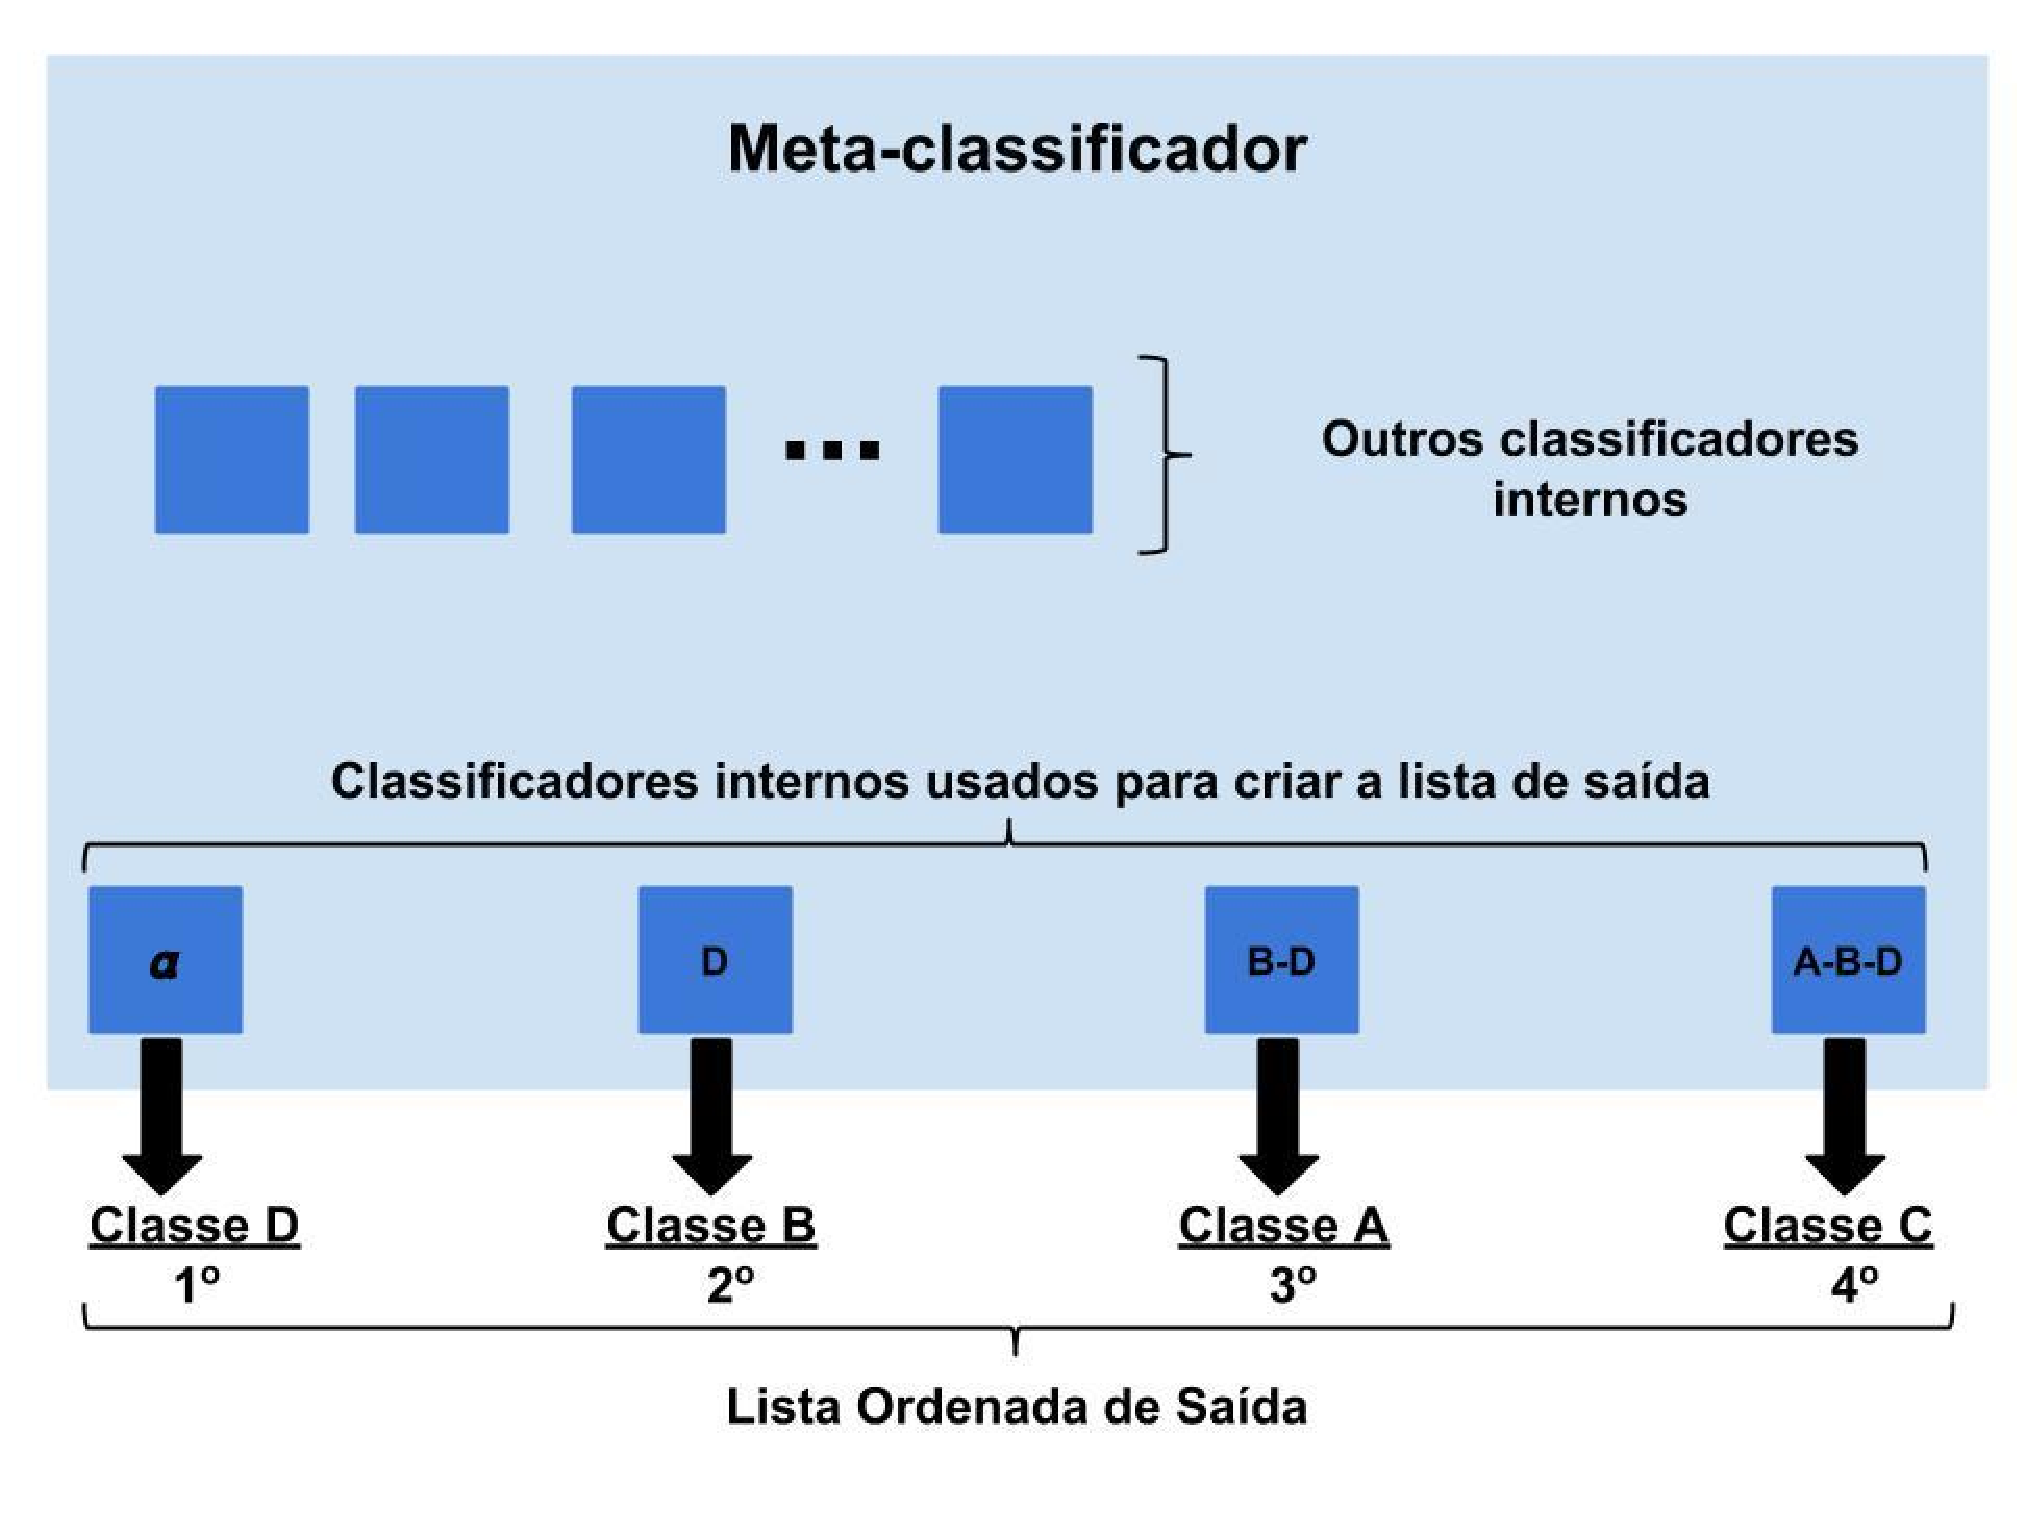
\includegraphics[width=\linewidth]{images/metodoproposto01.eps}
  \caption{Classificadores em cascata e lista de saída.}
  \label{fig:metodoproposto01}
\end{figure}

A Figura \ref{fig:metodoproposto01} ilustra como a lista de saída é gerada pelos classificadores internos.
Assuma que temos 5 classes distintas no conjunto de dados: A, B, C, D e E. 
No exemplo da Figura \ref{fig:metodoproposto01} queremos gerar uma lista de saída de tamanho quatro, logo quatro classificadores internos são utilizados. 
O classificador inicial (alfa),que foi treinado com o conjunto de treino completo, sempre gera o primeiro item de uma lista. 
O meta-classificador precisa então escolher um de seus classificadores internos para gerar um próximo item. 
Como a figura sugere, esta escolha depende de todos os elementos inseridos anteriormente na lista.
Repare na notação utiliza para nomear os classificadores, as letras depois barra "/" indicam as classes retiradas do conjunto de treino original para treinar aquele classificador.
Ou seja, o classificador /D foi treinado com um conjunto de treino filtrado de forma a excluir todas as instânicas da classe D, já o /BD exluiu aquelas das classes B e D e assim por diante.
Desta forma, o classificador /BD foi usado para gerar o terceiro elemento da lista por que as classes B e D já tinham sido colocadas na mesma.
Com isso o conjunto de treino utilizado para este classificador está livre da influência dessas classes.

\section{Funcionamento do Meta-classificador}

Seja \textit{T} o conjunto de treino do meta-classificador e \textit{v} o número de valores distintos que seu atributo classe pode assumir. 
Este conjunto será filtrado de formas diferentes e então utilizado para treinar os classificadores internos. 
Somente o classificador inicial, usado para gerar o primeiro elemento da lista de saída, é treinado com o conjunto de treino \textit{T} completo. 
Qualquer outro classificador interno é treinado com uma versão filtrada de  \textit{T}. 
De forma geral, o classificador que será usado para classificar o item da lista na posição \textit{k}, onde \textit{k} $<$ \textit{v}, deve ser treinado com um conjunto de treino filtrado \textit{k-1} vezes. 
Estas filtragens retiram sucessivamente do conjunto de treino as instâncias cujas classes já foram colocadas na lista.

No exemplo anterior, da Figura \ref{fig:metodoproposto01}, o classificador /ABD é usado para gerar o quarto elemento da lista.
Este classificador foi treinado com um conjunto filtrado 3 vezes (para retirar as instâncias com as classes A, B e D).
O processo de treinamento e classificação para um classificador interno é ilustrado na Figura \ref{fig:metodoproposto02}.

Note que o meta-classificador não foi desenvolvido para receber um conjunto de treino com uma lista ordenada no gabarito. 
Ele deve ser treinado com conjuntos que apresentam apenas um único valor no atributo classe.
Apos o treinamento com um conjunto de dados deste tipo o meta-classificador é capaz de gerar uma lista ordenada de classes para uma nova instância.

\section{Motivação}

A principal motivação para utilização deste método é a eliminação de ruído dos dados.
Como explicamos na seção anterior isso é feito através de filtragens sucessivas do conjunto de treino que eliminam as instâncias cuja classe já foi colocada na lista.
Para entender melhor a vantagem desta abordagem considere o caso de conjuntos de dados desbalanceados.
Isto é, que tem instâncias de diversas classes diferentes porém uma com a quantidade muito maior do que o restante.

\begin{figure}[h!]
  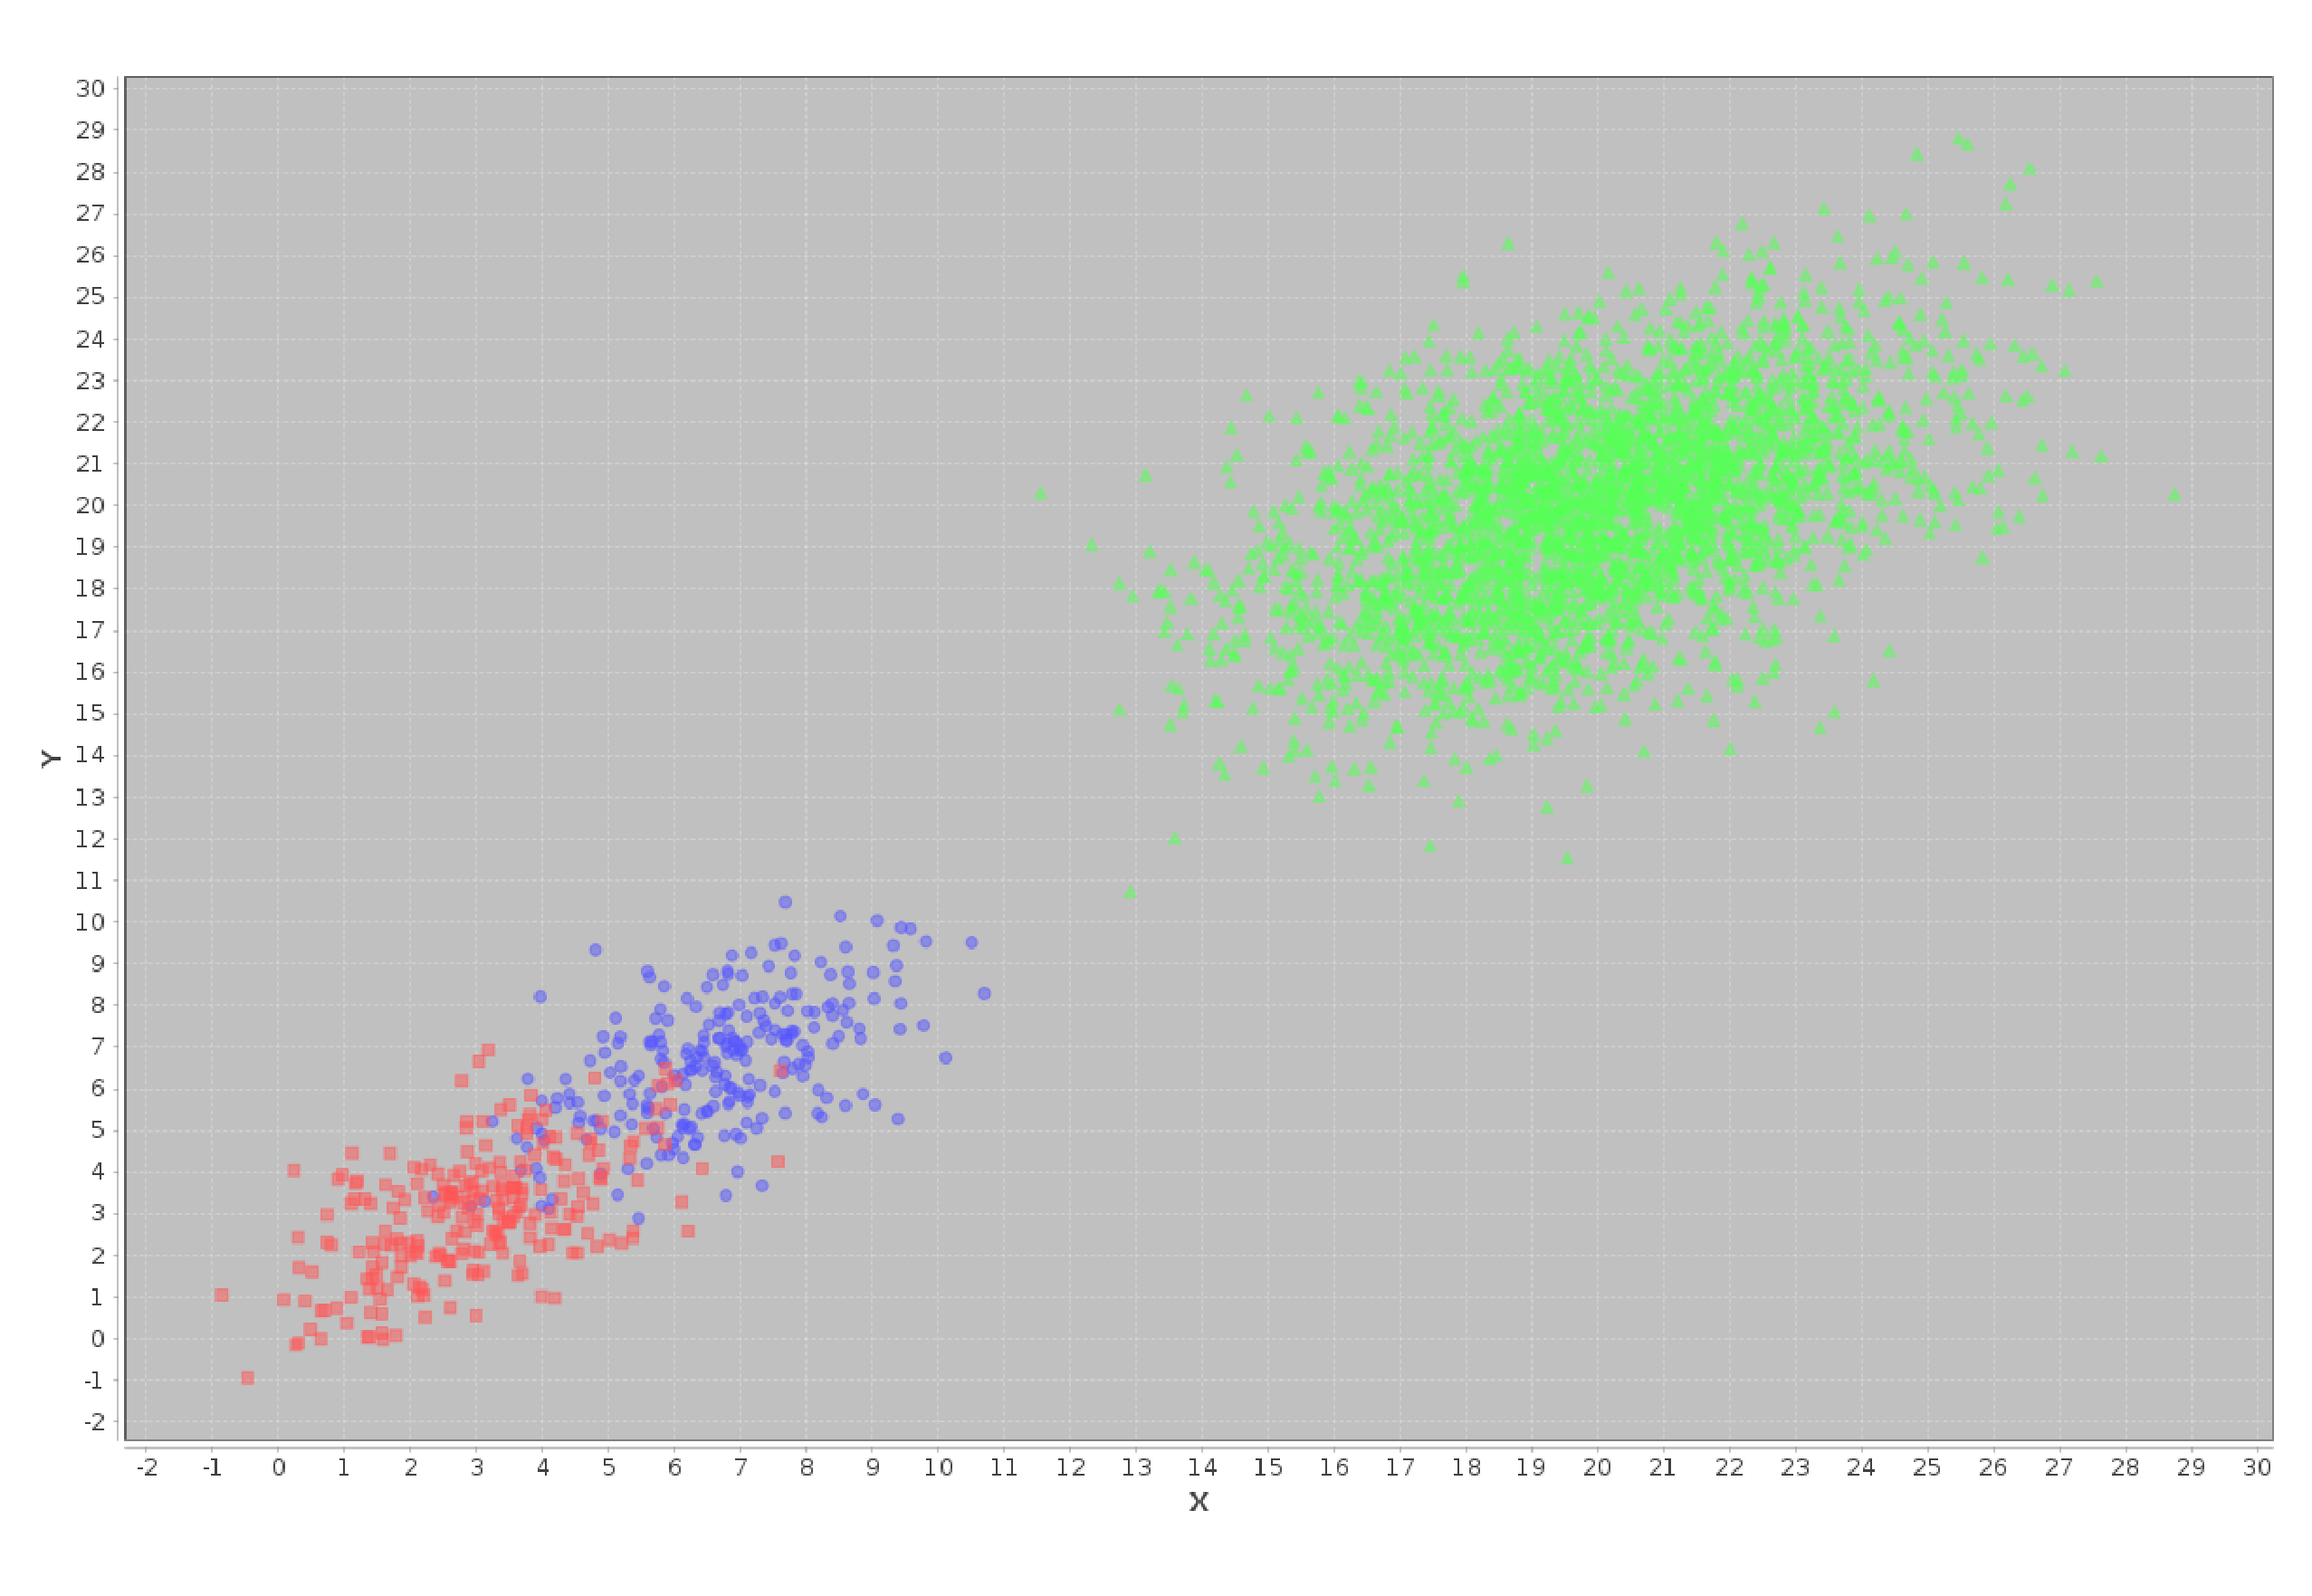
\includegraphics[width=\linewidth]{images/random_data_01.eps}
  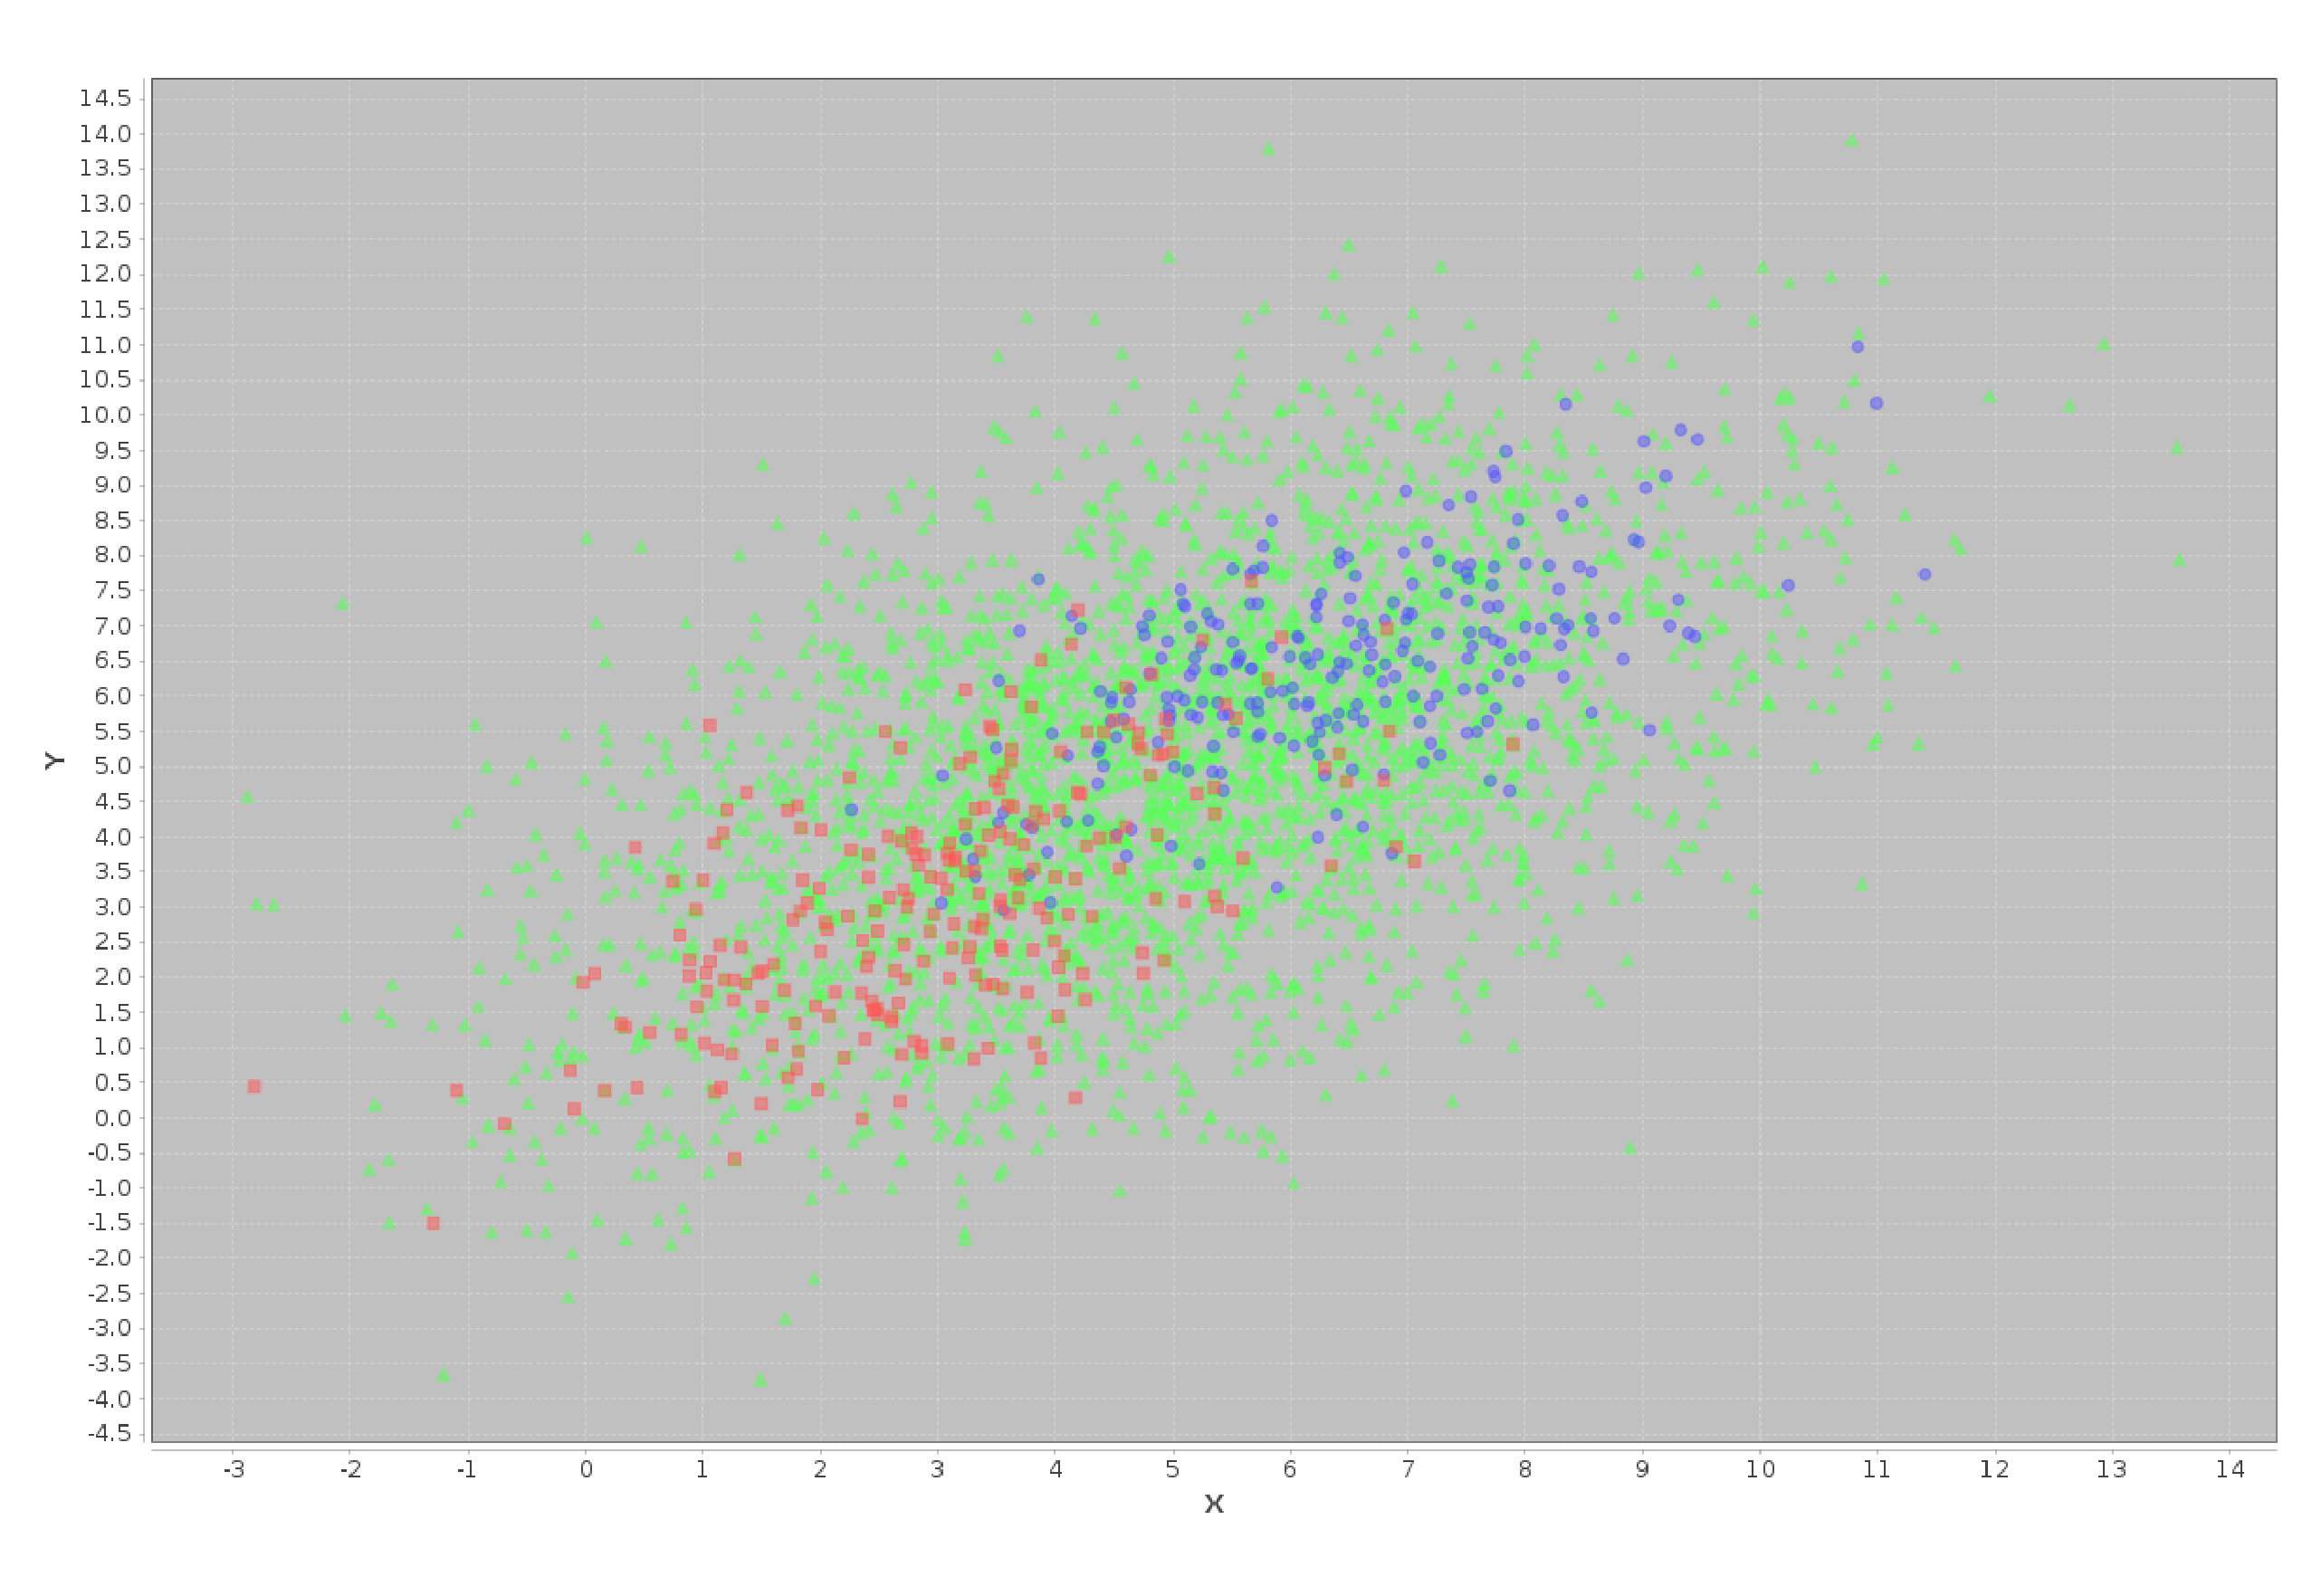
\includegraphics[width=\linewidth]{images/random_data_50.eps}
  \caption{Conjuntos de dados desbalanceados.}
  \label{fig:dadosdesbalanceados}
\end{figure}

A Figura \ref{fig:dadosdesbalanceados} ilustra dois conjuntos de dados desbalanceados gerados aleatoriamente.
Ambos tem a mesma quantidade de pontos, que estão agrupados de forma análoga em três grupos diferentes.
Considere que os pontos pertencentes ao mesmo grupo tem também a mesma classe, denotada pela cor: azul, vermelho ou verde.
Note que os dados são desbalanceados pois a classe verde tem uma quantidade de pontos muito maior do que as outras, são 3000 pontos verdes contra 250 azuis e 250 vermelhos.

Cada grupo de pontos foi gerado seguindo uma distribuição normal bivariada.
Apresentamos sua função densidade de probabilidade para um vetor aleatório \textit{(x,y)} a seguir.

\begin{equation*}
\resizebox{.99\hsize}{!}{
$f(x,y)=\frac{1}{2\pi \sigma _x\sigma _y\sqrt{1-\rho ^2}}\exp \left\{ -\frac 1{2(1-\rho ^2)}\left[ \left( \frac{x-\mu _x}{\sigma _x}\right) ^2-2\rho \left( \frac{x-\mu _x}{\sigma _x}\right) \left(\frac{y-\mu _y}{\sigma _y}\right) +\left( \frac{y-\mu _y}{\sigma _y}\right)^2\right] \right\}$
}
\end{equation*}

onde,

- $\mu$ é o vetor de médias dado por $\[ 
\left( \begin{array}{c}
\mu _x \\
\mu _y
\end{array} 
\right)\] $
 
- $\rho$ é a correlação entre x e y

- $\sigma$ remete à matriz de covariâncias $\Sigma=\[ \left( \begin{array}{cc}
\sigma _x ^2 & \rho \sigma _x \sigma _y \\
\rho \sigma _x \sigma _y & \sigma _y ^2 
\end{array} 
\right)\] $
\end{itemize}
\newline

No primeiro cenário da Figura \ref{fig:dadosdesbalanceados} os dados da distribuição que contem mais pontos (classe verde) estão afastados do restante.
Em contraste, no segundo cenário a média da distribuição de pontos verdes está entre os centros das distribuições de pontos vermelhos e azuis.
Depois de realizar testes com os dois conjuntos de dados percebemos que alguns classificadores, e.g. \textit{k nearest neighbors}, tem acurácias mais elevadas no primeiro cenário.
Notadamente, a presença da grande quantidade de pontos verdes próximos ao restante dificulta o aprendizado do classificador e piora o resultado final.

O metodo introduzido neste trabalho foi proposto no intuito de melhorar o resultado de casos como esse.
Suponha que queremos montar uma lista ordenada das cores mais prováveis para um ponto.
De acordo com o que já foi apresentado sobre o método, depois de selecionar um ponto verde para a lista, instâncias dessa classe serão eliminadas do conjunto de treino.
Desta forma o classificador utilizado para gerar o próximo elemento será treinado com um conjunto de treino sem a influência da classe mais numerosa (responsável pelo desbalanceamento).
Veremos em mais detalhes no capítulo \ref{chap:descricaodostestes} os resultados obtidos por nossa abordagem.

\section{Versões do método}
\label{sec:versoesdometodo}

O método proposto foi desenvolvido em duas versões: estático e dinâmico.


\subsection{Método Estático}

O método estático gera a priori todas os subconjuntos de classe que podem compor a lista de saída. 
Ele então treina todos os possíveis classificadores, cada um com sua versão filtrada do conjunto de treino, armazenando-os internamente.
Este conjunto de classificadores internos é efetivamente o modelo gerado pelo meta-classificador. 
Este pode ser usado então para gerar rankings ao receber novas instâncias. 

O pseudo-código a seguir descreve o procedimento de treinamento e classificação para a versão estática do método.
\\

\hline
\begin{center}
\textbf{Pseudo-Código: Funcionamento do Meta-Classificador}

\textbf{Versão Estática}
\end{center}
\hline
\hfill \break
-- \textit{Treinamento}\newline
Carrega o conjunto de treino completo\newline
Gera todas as possíveis combinações de classe sem repetições\newline
Para cada combinação de classe que foi gerada faça:

\quad Copia o conjunto de treino completo

\quad Remove da cópia os exemplos dessas classes

\quad Treina um classificador com este conjunto de treino modificado

\quad Armazena internamente o modelo gerado\newline
-- \textit{Classificação}\newline
Para cada item \textit{i} da lista de saída faça:

\quad Verifica as \textit{i-1} classes que já foram colocadas na lista de saída

\quad Recupera o modelo interno treinado sem essas classes

\quad Utiliza este modelo para gerar o \textit{iésimo} item da lista de saída

\hline
\hfill \break

Note que, quanto mais valores a classe do conjunto de treino original puder assumir, mais classificadores internos comporão o modelo do meta-classificador.
Sejam \textit{N} o número de classificadores geados pelo método estático, \textit{v} o número de valores de classe distintos no conjunto universo e \textit{k} o tamanho da lista que se deseja gerar. 
De forma geral, considerando que $\textit{k} \leq \textit{v}$, temos que:

\begin{equation*}

\centering
\textit{N} = \sum\limits_{i=0}^k \binom{v}{i}

\end{equation*}

A Figura \ref{fig:metodoproposto03} ilustra os classificadores internos gerados quando as possibilidades de valor de classe são A, B, C e D. Na figura as numerações não somente identificam cada classificador interno, elas denotam como o conjunto de treino foi filtrado para gerar aquele classificador. Além disso, a figura divide os classificadores internos em camadas. Um classificador que pertence a camada \textit{k} pode ser usado apenas para gerar um elemento na posição \textit{k} da lista de saída.

\begin{figure}[h!]
  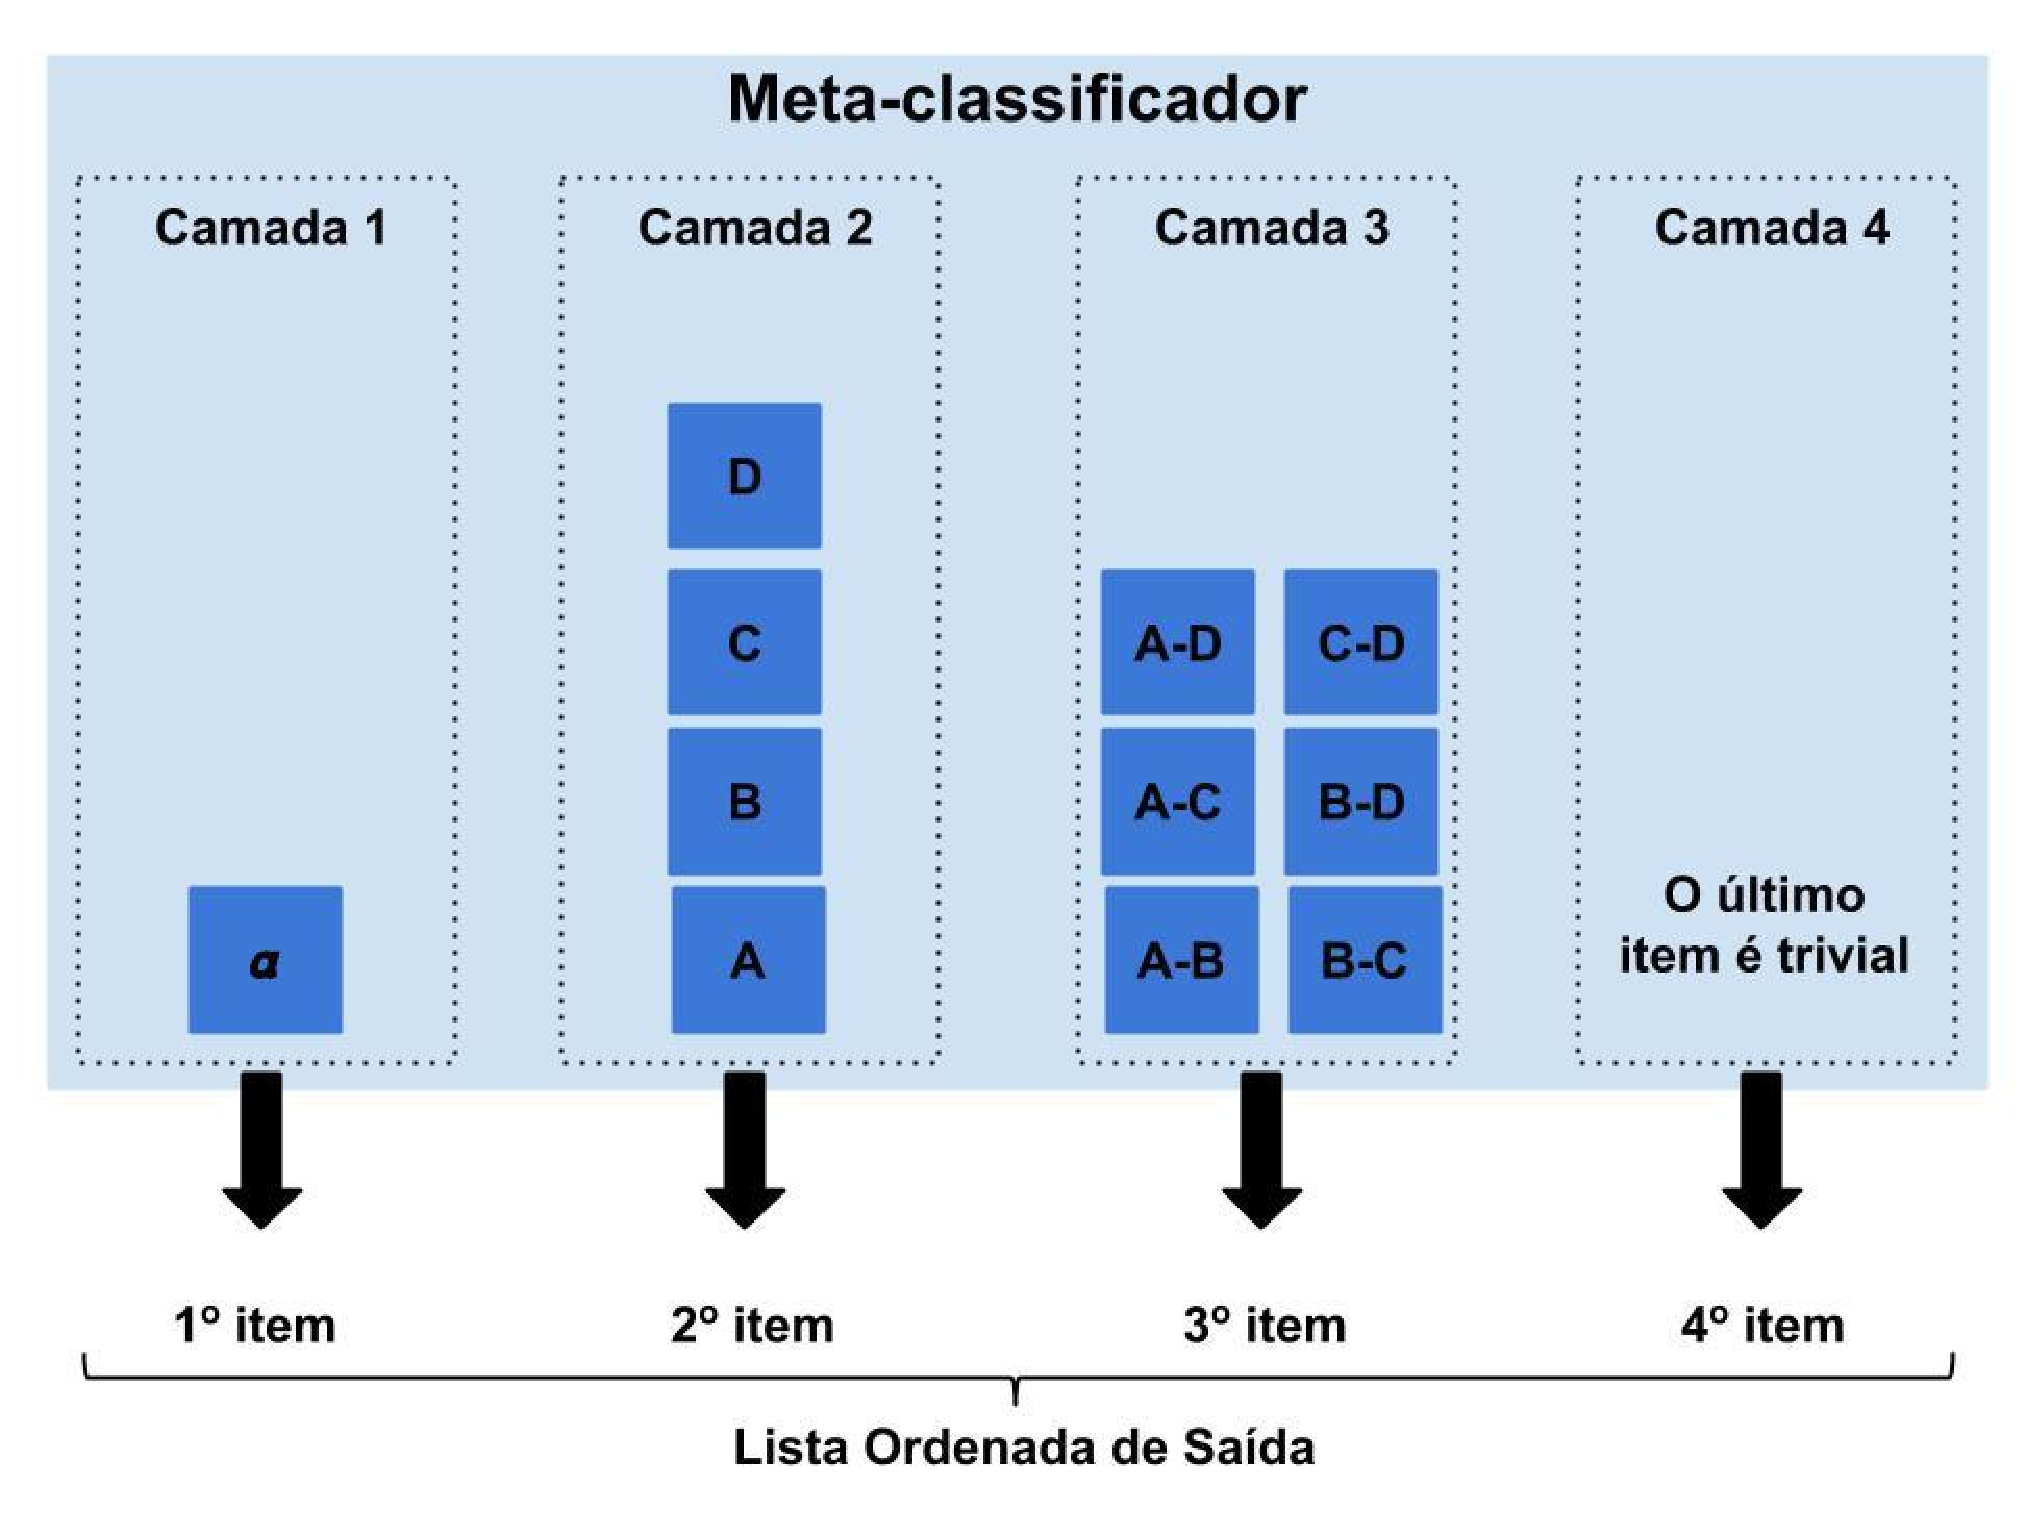
\includegraphics[width=\linewidth]{images/metodoproposto03.eps}
  \caption{Camadas de classificadores intenos.}
  \label{fig:metodoproposto03}
\end{figure}

A versão estática pode ser lenta durante a fase de treinamento, pois precisa treinar um grande número de classificadores antes de classificar qualquer nova instância. Por outro lado, uma vez treinado o modelo pode ser usado para classificar diversas novas instâncias rapidamente.

\subsection{Método Dinâmico}

O método dinâmico constrói o modelo na medida do necessário, treinando apenas os classificadores requeridos para a construção da lista de saída para a instância em questão. Ou seja, o modelo é treinado ao mesmo tempo que a classificação de instâncias é feita. De forma análoga ao método anterior, os classificadores são armazenados internamente a medida que são treinados. Desta forma, ao construir a lista de saída, os classificadores já treinados são reutilizados. Sendo assim, um mesmo classificador nunca é treinado mais de uma vez. 

O pseudo-código a seguir descreve o procedimento de treinamento e classificação para a versão dinâmica do método.
\\

\hline
\begin{center}
\textbf{Pseudo-Código: Treinamento de Classificador Interno}

\textbf{Versão Dinâmica}
\end{center}
\hline
\hfill \break
Carrega o conjunto de treino completo\newline
Para cada item \textit{i} da lista de saída faça:

\quad Verifica as \textit{i-1} classes que já foram colocadas na lista de saída

\quad Copia o conjunto de treino completo

\quad Remove da cópia os exemplos das \textit{i-1} classes já incluidas na lista

\quad Treina um classificador com o conjunto de treino modificado

\quad Armazena internamente o modelo gerado

\quad Utiliza este modelo para gerar o \textit{iésimo} item da lista de saída
\hline
\hfill \break

\begin{figure}[h!]
  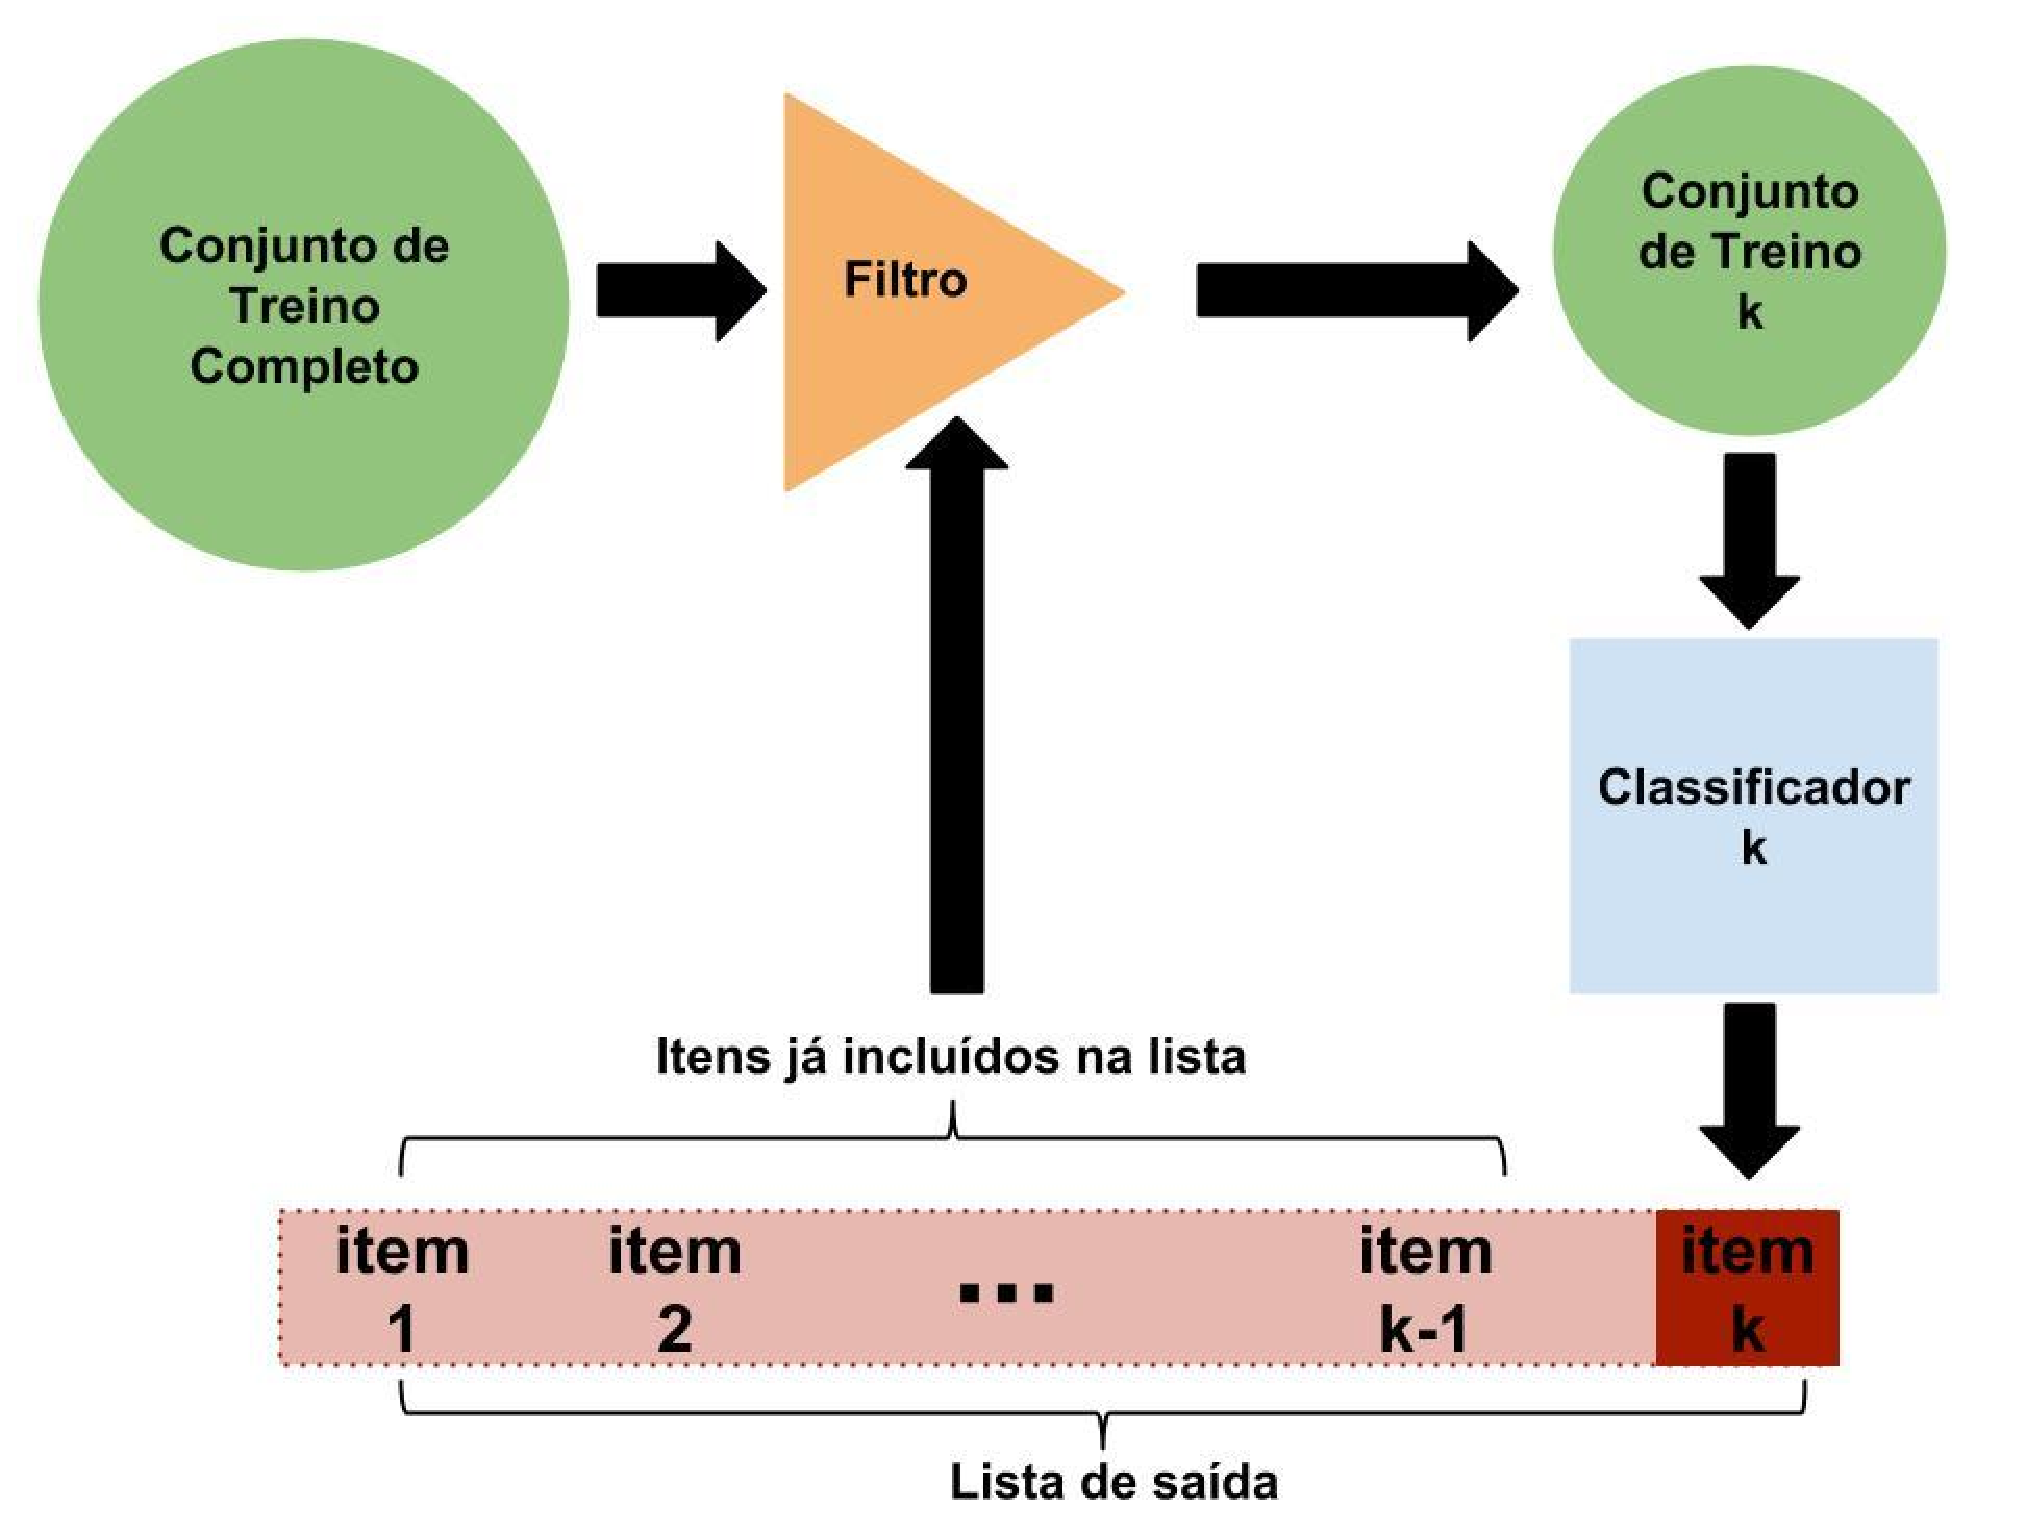
\includegraphics[width=\linewidth]{images/metodoproposto02.eps}
  \caption{Filtragem do conjunto de treino e treinamento de um classificador.}
  \label{fig:metodoproposto02}
\end{figure}

Esta segunda versão tende a ser mais rápida do que a anterior, visto que não precisa treinar todas as possíveis combinações de classificadores a priori. Entretanto, como o treinamento do modelo é feito ao mesmo tempo que a classificação de instâncias, o tempo de classificação da versão dinâmica é maior do que a versão estática. 

Concretamente, sejam \textit{k} o tamanho da lista de saída, \textit{M} o tempo médio de treinamento de um classificador interno e \textit{t} o tempo médio de classificação de um único ítem por um classificador interno já treinado. Note que tipicamente temos que $ \textit{M} >> \textit{t} $. Considere o caso onde o meta-classificador ainda não tem um classificador interno treinado. Usaremos este como limite superior para o tempo de construção da lista de saída para uma nova instância. Este tempo é calculado por $ \textit{T} = \textit{k}\left(\textit{M} + \textit{t}\rigth) $. Por outro lado, o limite inferior para o tempo \textit{T} ocorre no caso onde o meta-classificador já treinou a priori todos os classificadores internos necessários na construção da lista de saída de uma nova instância. Neste caso temos $ \textit{T} = \textit{k}\textit{t} $.

\section{Vantagens e Desvantagens do método}

O método proposto tem a versatilidade de permitir o uso que qualquer classificador internamente. Além disso, as sucessivas filtragens do conjunto de treino removem as instâncias com classes que não são mais pertinentes para construção da lista de saída. Estas duas carcterísticas podem contribuir para melhoria do resultado final com (1) a escolha do classificador interno mais adequado e (2) a remoção de ruído do conjunto de treino.

Uma desvantagem deste método é o alto custo computacional do treinamento dos classificadores internos, tanto em processamento quanto em memória. Dependendo da quantidade de valores de classe, o modelo do meta-classificador pode requerer o treinamento de centenas ou milhares de classificadores internos. Esta desvantagem pode vir a ser proibitiva para a versão estática do método. 

A versão dinâmica mitiga este problema pois treina os classificadores internos somente quando são necessários. Desta forma ela economiza processamento em comparação com a versão estática. Ainda assim, pode ser necessário grandes quantidades de memória durante a execução do programa. Com isso podendo ser inviável a execução do mesmo na maioria das máquinas. Portanto, um gerenciamento de memória foi desenvolvido. Este garante que a memória alocada não superará um limiar máximo, especificado no momento da execução do programa.

A solução desenvolvida em Java para implementar o método proposto mantém um conjunto interno de objetos, que são classificadores já treinados. Com o gerenciamento de memória, sempre que a memória alocada pelo programa atingir um determinado patamar \textit{M}, um número \textit{c} de classificadores é removido do conjunto. Estes classificadores são removidos do menos usado para o mais usado. Tanto \textit{M} quanto \textit{c} podem ser ajustados pelo usuário no momento da execução do programa. Note que para que isto funcione \textit{M} deve ser menor do que a quantidade máxima de memória disponível. Desta forma, em um momento posterior a exclusão destes classificadores internos, o \textit{Garbage Collector} do Java liberará a memória. Com isso está garantido que o programa não poderá ficar com memória insuficiente para sua execução.
